\documentclass{standalone}
% preamble: usepackage, etc.
\begin{document}

\chapter{复杂图推理中的知识表示}
\section{概况}
本章主要是介绍图同构推理引擎在复杂图推理中的知识表示问题,主要分为
两大模块,一个是初等数学领域概念知识图谱的构建,另一方面是实例化
定理库的构建。其中概念知识图谱的构建从知识图谱构成、知识图谱存储、
知识图谱的应用三个方面介绍;实例化定理库的构建则从定理来源、定理库
创建、定理书写规范、定理的应用四个方面介绍。总体关系图如图3-1所示。

\begin{figure}[htbp]
	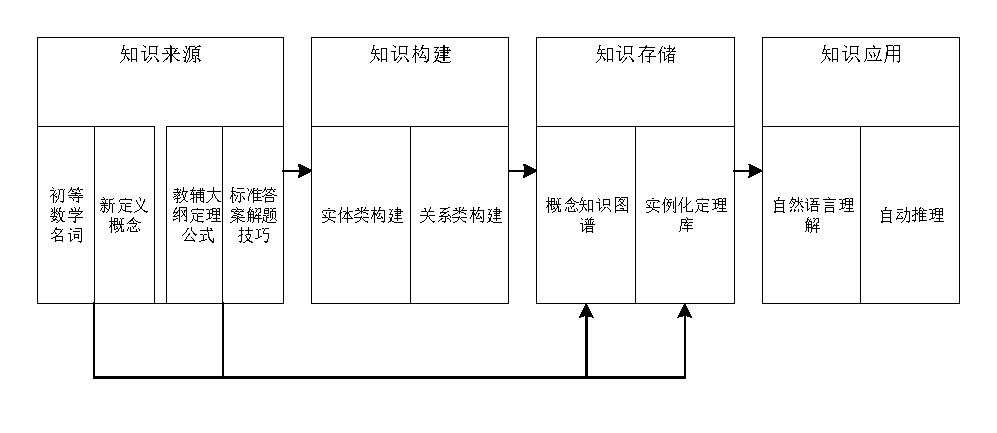
\includegraphics{知识表示.pdf}
	\caption{知识表示关系图}
	\label{知识表示}
\end{figure}
\section{概念知识图谱的构建}
\subsection{知识图谱构成}
知识图谱是用一个逻辑上的图去表征语义,这个图可以是连通的,也可以是
非连通的。本文中构建的初等数学领域的概念知识图谱就是有一些离散图
组成的逻辑上的大图。无论是离散图还是逻辑上的图,它们的最小组成单位
都是三元组结构,本文中设计的图同构推理引擎的最小推理结构就是知识
图谱中的三元组。三元组则是由两个实体和它们之间的关系构成的,实体
和关系又是三元组的最小组成单位。例如,”三角形ABC与三角形DEF相似“,
解析成三元组结构为(三角形,相似关系,三角形),这里的头尾实体均为
”三角形“,关系为”相似关系“。这里为了描述方便起见,以实体和关系的
类型字段表示,但对于后续推理来说,实体类和关系类的字段和属性信息
远丰富的多。接下来详细介绍本文如何构建实体类和关系类。

(1)实体类的构成
本文中实体都是来源于初等数学中基本概念、名词,如”函数“实体、”向量“
实体、”数列“实体、”双曲线“实体等。当前构建的实体类共236个,为了保证
实体类的可扩展性和灵活性,在最初的架构设计上采用了”开闭原则“和应用
Java语言的继承、多态以及反射的思想,即我们构建出一个抽象实体类
AbstractData,在AbstractData中添加共有的属性字段,以及相关的
函数方法,再让所有的具体实体类继承AbstractData,这样的好处有
两点:第一点可以做到很好的扩展性,可以随时添加新的实体类;第二点
方便编码,当不知道是哪个实体类时,在编译时期可以直接创建抽象父类
实体类,再利用反射技术指向不同的子类对象。

抽象实体类除了上文中描述的作用,它的一些字段在推理中也至关重要。
如表3-1是AbstractData抽象实体类的具体属性字段表。
\begin{table}[h]
	\caption{抽象实体的属性表} 
	\begin{tabular}{|c|c|c|} 
		\hline  
		属性名 & 中文含义 & 描述 \\
		\hline 
		EntryName & 实体名 & 用于命名实体,在知识图谱和类人解答过程中显示\\  
		\hline  
		Id & 实体的唯一标识 & 来唯一标识实体 \\  
		\hline  
		TypeName & 实体类型 & 实体的类型应用于三元组匹配 \\  
		\hline 
		Knowledge & 新知识 & 存储知识更新阶段的新知识 \\  
		\hline 
		Used & 是否使用过 & 用于记录实体在遍历时是否已经出现,避免重复 \\  
		\hline  
	\end{tabular}
	\label{tablea}
\end{table}

(2)关系类的构成
关系是表示两个实体之间的关联,因此关系类中首先会记录它所关联的
头尾实体的信息,这里为了区分关系名和实体名,自然语言处理中会
统一给抽取的关系命名加上”Relation“后缀,如首项关系”FirstItem
Relation"。为了保证图推理引擎的匹配精确度,关系类构建的需要
符合以下几条准则:

1)关系的命名尽量规范,头尾实体名加上“Relation"后缀;

2)关系名的唯一性,若出现关系名重复,代码运行时会有反射异常;

3)关系构建尽量精细化,如”点在直线上“,”点在圆上“,我们应当
构建”PointOnLineRelation","PointOnCircleRelation",而不是
都构建成“OnRelation”。

同样的,与实体类建模相同的是,所有的具体关系类也都继承于同一个
抽象父类AbstractRelation。与AbstractData一样,AbstractRelation
也有关系特有的一些属性值,不同的属性值在推理中发挥着不同的用途。
下表3-3是AbstractRelation抽象实体类的具体属性字段表。

\begin{table}[h]
	\caption{抽象关系的属性表} 
	\begin{tabular}{|c|c|c|c|} 
		\hline  
		属性名 & 中文含义 & 描述 & 数据类型\\
		\hline 
		RelationName & 关系名 & 用于命名关系,在知识图谱和类人解答过程中显示
		& String\\  
		\hline  
		RelationId & 关系的唯一标识 & 来唯一标识关系 
		& String\\  
		\hline  
		IsSelfCircle & 是否自环关系 & 应用于自环映射判断
		& boolean \\  
		\hline 
		FullName & 关系全路径名 & 通过全路径名来发射到相应的具体关系类
		& String \\  
		\hline 
		Order & 关系序 & 用于对相同关系的三元组重排序
		& Integer \\  
		\hline  
		IsSameGroupe & 是否同组 & 用于消除假组合降低组合次数
		& Integer \\  
		\hline 
		RelProperties & 关系属性 & 用于支持属性匹配和更新
		& Map \\  
		\hline 
		IsConclusion & 是否结论三元组 & 用来标记三元组类型,区分
		条件三元组和结论三元组
		& Integer \\  
		\hline 
		CreateBranch & 创建分支 & 判断该关系是否触发了分支
		& boolean \\  
		\hline 
		Knowledge & 新知识 & 新知识为关系的属性
		& String  \\  
		\hline 
	\end{tabular}
	\label{tablea}
\end{table}

\subsection{知识图谱存储}
概念知识图谱就是由这些实体类和关系类通过转换成图谱中的节点和关系,
然后存储在Neo4j图数据库中。Neo4j是一种图数据库,图中节点可以存储
实体类相关信息,Neo4j支持的数据格式是字符串以及字符串数组,对于
每一对属性值是k-v键值对存储的形式。同样的,图中节点之间的边就是
用来存储关系类的相关信息。这里特别说明,由于Neo4j图数据库数据
存储不支持对象存储,这对后面有些属性作为对象存储并不是友好兼容,
例如,“两直线相交于点P”这是三元关系的描述,如何在知识图谱中表征
三元关系,有两种处理方式。第一种解构成一个三元组(直线,相交关系,直线)
,其中实体点P作为相交关系的属性存储;第二种是将三元关系转换成
多组两元关系,(直线,相交关系,直线),(点,在直线上关系,直线),
(点,在直线上关系,直线),这样便实现了多元关系的存储。在后续的
推理中我们大多数使用第二方式去存储多元关系。如图3-2(a)和如图3-2(b)
分别是三元关系的知识图谱两种不同存储示意图。
***************************
\subsection{知识图谱的应用}
本文中初等数学知识图谱主要应用在自然语言理解的关系抽取中和后端
解题的实例化子图。自然语言理解是整个解题系统求解过程的第一步,
后端的推理也是依赖于前端自然语言理解的结果,因此要求自然语言
理解要尽可能地命名体实别准确以及保证这些实体之间的关系抽取的
准确度。初等数学概念知识图谱便给关系抽取提供一定的支撑,首先
命名体识别是自然语言理解的第一步,命名体识别出来的实体则对应
于知识图谱中的实体节点。自然语言理解和知识图谱是个相辅相成、
相互完善的过程:当出现自然语言理解识别出的实体在知识图谱中
没有,需要在知识图谱中补充;当自然语言理解识别的实体于
知识图谱中的不一致,需要对自然语言理解实体命名做修正。
进一步,对于关系抽取的第一步,输入任意两个实体,去概念
知识图谱中反查出这两个实体所包含的所有关系,最终抽取的
关系必须在这组关系集合中,因此知识图谱的构建对自然语言
理解至关重要。

后端解题中同样需要依赖于知识图谱。本文构建的是一个图
推理引擎,推理引擎的入口就是自然语言理解实例化出来的子图,
其中包括题目子图和规则子图。无论是题目子图和实例化子图都
必须能在概念图谱中包含其所有的实体和关系,如果在概念图谱
中找不到子图对应的实体或者关系,推理引擎则会抛出反射异常,
需要自然语言理解或者知识图谱做相应的修正和补充。

\section{实例化定理库的构建}
\subsection{定理来源}
本文要构建的是初等数学领域的实例化定理库,定理的范围是初等
数学领域,定理的来源于三个部分:第一部分是目前初中、高中的
数学教材上的定理以及公理,同时参考市面上主流教辅书籍(如
《高中数学知识清单》【】)和互联网上相关的信息;第二部分
是从标准答案的解题过程中抽取相应的解题方法、解题技巧,
为了保证自然语言理解的可靠性,标准答案会做些微调,尽量
保证标准答案中描述的实体类型明确,可以是一个短句作为一个
实例化定理,也可以是多个短句组合成一个实例化定理。第三部分
是表达式变形,表达式的恒等变形,合并同类项,拆分移项等一系列
操作转化成实例化定理。

为了方便定理库的管理和提升推理引擎对定理库的搜索效率,对定理进行
分类收集、分类构建、分类存储。目前基于初等数学题型特征,将定理
分成五个大类:函数、数列、向量、解析几何、平面几何。下表3-4(a)、
3-4(b)、3-4(c)、3-4(d)、3-4(e)分别是五个类型定理公式表。

\begin{table}[h]
	\caption{函数实例化定理} 
	\begin{tabular}{|c|c|c|} 
		\hline  
		定理标签 & 定理名称 & 描述 \\
		\hline 
		rKwkWrig & 函数与坐标轴相交 
		& \makecell[l]{函数$f(x)=g(x)$与$x$轴只有$n$个公共点,\\则$\#publicPointOfFunction\#f(x)=g(x)\&n$}\\  
		\hline  
		qyZkFwKa & 函数到曲线 
		& \makecell[l]{已知函数$F$的曲线为$E$,\\则曲线$\#Func2Curve\#F$}\\  
		\hline  
		XkylPYoG & 函数单调区间
		& \makecell[l]{已知函数$f(x)=g(x)$,\\则$f(x)=g(x)$的单调区间为$\#GetFuncMonoItv\#f(x)=g(x)$}\\ 
		\hline 
		oOakjOWd & 函数有零点 
		& \makecell[l]{若函数$f(x)$有零点$rsa$,\\则不等式$\#haveZeroOfFunction\#f(x)$}\\ 
		\hline 
		IOekuEOt & 函数求导 
		& \makecell[l]{已知函数$f(x)=g(x)$,\\$f(x)=g(x)$的导函数为$\#diffOfFun\#f(x)=g(x)$}\\  
		\hline  
		zsBlBQjc & 求函数周期 
		& \makecell[l]{已知函数$f(x)$,\\则$f(x)$的最小正周期为$\#CalPeriod\#f(x)$}\\ 
		\hline  
		JCekuEOt & 求反函数 
		& \makecell[l]{已知函数$f(x)=g(x)$,\\$f(x)=g(x)$的反函数为$\#inverse\#f(x)=g(x)$}\\  
		\hline  
		UQbkuGfC & 计算函数最大值
		& \makecell[l]{已知函数$f(x)=g(x)$,\\则$f(x)$的最大值为$\#CalculateMaxValueOfFunc\#f(x)$}\\  
		\hline  
		 DegkuGfC & 计算函数最小值 
		& \makecell[l]{已知函数$f(x)=g(x)$,\\则$f(x)$的最小值为$\#CalculateMinValueOfFunc\#f(x)$}\\  
		\hline 
	\end{tabular}
	\label{tablea}
\end{table}


\subsection{定理库创建}
每条实例化定理创建是将上述定理公式经过自然语言理解生成三元组结构
的json字符串,后端接受到前端实例化定理的json会生成定理知识图
并存储在neo4j图数据库中,定理库则是将所有搜集的定理公式均转成
实例子图存储在数据库中。目前实例化库的实例化总数为323条,其中函数
107条,数列89条,向量38条,解析几何101条,复数21条。

实例化定理文本和题目文本在自然语言输入的时候是有所区别的。自然语言
提供”type“的属性字段,当”type“输入为0时,表示输入的时实例化定理。
定理的文本输入分成两个部分,前提条件和结论分开输入,前提条件三元组
和结论三元组是通过关系中属性字段”isConclusion"区分,当”isConclusion"
为2时是结论三元组,其他取值为前提条件三元组。
除了”type“字段,实例化定理还包含另外两个个标注字段:”instantiatedLevel“
、”instantiatedCategory“、”instantiatedDescription“。其中,
”instantiatedLevel“字段含义代表该实例化定理的优先级,范围值为0-1000,
0代表优先级最高,数值越大优先级越低。”instantiatedCategory“表示
实例化定理类别,范围值为1-8,1代表函数,2表示向量,3表示数列,
4表示解析几何,5表示复数,6表示平面几何,7表示立体几何,8表示
表达式变换。通过自标注实例化属性字段,更加丰富了实例化定理的内容,
并具体应用后续的自动推理和知识点标注中。实例化定理的详细标注字段
如表3-5所示。 

\begin{table}[h]
	\caption{实例化定理属性字段} 
	\begin{tabular}{|c|c|c|} 
		\hline  
		属性字段 & 描述 & 用途 \\
		\hline 
		type & 输入类型 & 用于区分实例化定理和题目输入\\  
		\hline  
		instantiatedLevel & 实例化优先级 & 推理引擎的实例化选取 \\  
		\hline  
		instantiatedCategory & 实例化类别 & 实例化分类器 \\  
		\hline 
		instantiatedDescription & 实例化描述 & 类人解答显示和知识图谱显示 \\  
		\hline 
		instantiatedKnowledge & 知识点 & 记录推理路径中使用的知识点 \\  
		\hline  
		instantiatedKnowledgeWeightsedge & 知识点权重 & 知识点的优先级 \\  
		\hline  
		IsConclusion & 是否结论三元组 & 区分结论三元组和条件三元组 \\  
		\hline 
	\end{tabular}
	\label{tablea}
\end{table}

\subsection{定理书写规范}
上文中介绍了实例化定理的来源,为了保证推理引擎的简单性和统一性,
需要对实例化定理进行规范化和标准化书写。首先,实例化定理是分成
两个部分,前提条件和结论。其中,前提条件就是原始的定理文本描述,
是实例化定理参与匹配的部分;结论部分是需要部分人工参与书写,它
是推理引擎产生知识的依据,即当该实例化匹配成功时,推理引擎会解析
定理结论部分,然后触发相应的符号计算服务,产生定理知识并依据不同
的知识更新策略,将新知识插入到原有的知识库中,进行下一轮的知识迭代。
因此推理引擎对实例化结论部分的书写提出了以下准则:

(1)标准化实例化定理结论部分由三个部分组成:操作函数、定理公式、形式化
参数。操作函数是触发定理产生新知识的一组动作,操作的对象就是定理公式
以及形式参数置换后的具体参数,在书写时使用“\#”将操作函数进行区分,操作
函数有时可以省略,当省略时,引擎会默认添加“simp”操作函数表示化简操作;
定义公式是操作函数操作的对象之一,它可以是书中的定理公式、等价变形或者
表达式变换,例如求等差数列前n项的通项公式“$a_n=a_1+(n-1)*d$","$x^2+2*x*y
+y^2=(x+y)^2$"等都属于定理公式的范畴;形式化参数指的是定理中抽象化参数,
不参与具体计算,需要注意的是定理公式和形式化参数之间是”:“隔开,而参数
于参数之间是”\&“符号隔开。最终,完整的一条实例化定理的结论部分便书写完成。
如求等差数列通项公式的实例化定理结论为:”\#simp\#$a_n = a_1+(n-1)*d$:$a_1$\&$d$“

(2)如表3-3列举了常见的操作函数表
\begin{table}[h]
	\caption{操作函数表} 
	\begin{tabular}{|c|c|c|} 
		\hline  
		操作函数名 & 参数表 & 描述\\
		\hline 
		Simplify & \makecell[l]{String expression,\\List<String> conditions}
		 & 在指定条件下化简表达式\\  
		\hline  
		Solve & \makecell[l]{List<String> equations ,\\List<String> vars} 
		& 解单个方程或者方程组 
		\\  
		\hline  
		rsolve & \makecell[l]{List<String> condition} 
		& 解递归方程
		\\  
		\hline 
		union & \makecell[l]{String setA,\\String setB} 
		& 有限集合的并集
		\\  
		\hline 
		intersect & \makecell[l]{String setA,\\String setB} 
		& 有限集合的交集
		 \\  
		\hline  
		sumOfPreNminus1Items & \makecell[l]{String formula} 
		& 连加数列求和
		 \\  
		\hline 
		VectorialAngle & \makecell[l]{String vector1,\\String vector2}
		& 计算向量夹角
		 \\  
		\hline 
		getCosOfVectorAngle & \makecell[l]{String vector1, \\String vector2}
		& 计算向量夹角余弦值
		\\  
		\hline 
		CalculateMaxValueOfFunc & \makecell[l]{String funcAndConditions, \\boolean isMax}
		& 在定义域范围内,计算函数最大值
		\\  
		\hline 
		CalculateMinValueOfFunc & \makecell[l]{String funcAndConditions, \\boolean isMin}
		& 在定义域范围内,计算函数最小值
		\\  
		\hline 
		definitionOfFun & \makecell[l]{String function, \\String var}
		& 计算函数定义域
		\\  
		\hline 
		extreme2Equation & \makecell[l]{String function, \\String extremePoint}
		& 根据函数极值点,生成导函数为0的方程
		\\  
		\hline 
		diffOfFun & \makecell[l]{String function,\\String var}
		& 函数求导
		\\  
		\hline 
		PluralPoint & \makecell[l]{String express}
		& 复数求对应点
		\\  
		\hline 
		PluralReal & \makecell[l]{String express}
		& 复数求实部
		\\  
		\hline 
		PluralImag & \makecell[l]{String express}
		& 复数求虚部
		\\  
		\hline 
		equationDiscriminant & \makecell[l]{String equation}
		& 生成方程判别式
		\\  
		\hline 
		slopeEquation & \makecell[l]{String function}
		& 求形如y=f(x)的斜率
		\\  
		\hline 
	\end{tabular}
	\label{tablea}
\end{table}

(3)上文中介绍过形式化参数是不直接参与计算的,主要是完成接下来形参到实参
的置换,因此实例化中的参数书写也需遵循一定的规则。

3.1)变量名的置换。所谓变量名置换,即只对具体题目参数中的名称进行替换。
如,实例化中参数为点P,题目中具体参数为点A=(1,2),变量名置换法则是
只替换A=(1,2)的变量名”A“,返回的置换结果是P=(1,2)

3.2)全称替换。有些情况下,需要获取到原始题目的所有参数信息,而不是只
进行变量名的替换,需要注意运算符两边变元数相同,全称替换在函数中应用
较为广泛。例如,实例化中参数是$f(x)=g(x)$,题目中具体参数为$h(x)=a*x^2-b$,
因为运算符”=“两边的变元数相同,发生的事全称置换,置换后的结果是保留原始
题目参数$h(x)=a*x^2-b$;若实例化参数改写成函数$f(x)$,则发生的置换是变量名
置换,置换结果为$f(x)=a*x^2-b$

3.3)变元置换。变元置换是指对表达式中的变量进行一一映射,从而产生一组
或多组轮换关系。变元置换在置换策略中应用广泛,在完成变量抽取后,对变量
进行轮换映射参与后续的计算模块。本文中的变元置换具体表现为:数列角标的
置换、函数的自变量置换、系数置换等。例如,$f(x)=a*x^2+b*x+c$和
$f(x)=x^2+9*x-3$所对应的一组轮换映射为\{a=1,b=9,c=-3\},$a_m+a_n=p$和
$a_3+a_5=0$所对应的一组轮换映射为\{m=3,n=5,p=0\}

\subsection{定理的应用}
在整个问题求解系统中,解题是最核心的部分,是系统的功能需求和第
一步目标,而解题的核心部分是推理引擎,图推理引擎设计的驱动依据就是
实例化定理。定理驱动方式分为两种,一种是针对所有实例化定理采用循环
驱动,这是一种外部驱动;第二种针对单个实例化,是内部驱动方式。图推
理引擎会对实例化定理子图进行解构,将实例化子图拆分成逻辑上独立的两
个子图:条件子图和结论子图。其中,条件子图作为引擎匹配的依据,结论
子图作为引擎产生新知识以及如何插入到原知识库的依据。当匹配成功时,
才会触发引擎对结论子图的处理,否则会进入到外部循环驱动,进入到
下一条规则的匹配。因此定理是引擎解题的重要依据,包括如何在定理库
中搜寻一条或多条解题路径。

实例化定理除了在解题中应用,同样应用在知识点标注上。在自然语言
处理过程中,对实例化定理添加了三个个字段”instantiatedKnowledge“,
”instantiatedKnowledgeWeights“,”instantiatedDescription“。
”instantiatedKnowledge“代表该实例化定理涉及到的相关知识点,
”instantiatedKnowledgeWeights“标记该知识点的权重值,当一个
实例化包含多个知识点信息时,可以通过知识点权重来确定知识点的优先级。
知识点来源于初高中教材的大纲知识点,由于一条定理可能包含多个知识点,
因此字段”instantiatedKnowledge“设计成List<String>数据结构。
”instantiatedDescription“表示实例化的定理名称,主要是用于后续解答过程的答案
输出,同时实例化标签label加上定理名称便可形成对定理的唯一标识。
解题是知识点标注和类人过程输出的基石和前提,它们之间的关系具体
表现为:推理引擎在对实例化定理库进行搜寻的过程中构建解题的
定理树,对定理树进行回溯查询得到类人解答过程,定理树是记录
解题过程中所使用的实例化定理之间的逻辑关系,通过”instantiatedKnowledge“
字段输出本题涉及到的所有知识点内容。


\section{本章小结}
本章首先研究了时域积分方程时间步进算法的阻抗元素精确计算技术,分别采用DUFFY变换法与卷积积分精度计算法计算时域阻抗元素,通过算例验证了计算方法的高精度。

\end{document}
